\documentclass[11pt]{myclass}
\usepackage[margin=1in]{geometry}
\usepackage{mathptmx}
\usepackage{color}
\usepackage{hyperref}
\usepackage{verbatim}
\usepackage{amssymb}
\usepackage{algorithm, algorithmic}


\newcommand{\breg}{\ensuremath{D_\phi}}
\newcommand{\sbreg}{\ensuremath{D_{s\phi}}}
\newcommand{\eps}{\varepsilon}

\title{CS 5350 Final Project Report}
\author{Vishay Vanjani, Alex Clemmer, \textit{Godzillasaurus Rex}}
%\date{} % Activate to display a given date or no date (if empty),
         % otherwise the current date is printed 

\begin{document}
\maketitle

\section{System Components}

\subsection*{Incident Slot Predictor}
For this slot we used about 50 manually crafted patterns. Each pattern was associated with a “incident type” and a Score. The classifier selected the “incident type” with max score to make the prediction. Our scoring system gave scores according to 1) relevance of pattern 2) frequency of pattern . For example the patterns for bomb (“bombed” or “bomb”) had lower scores than patterns for arson (“set fire to”).

\subsection*{Pattern Extraction using AutoSlog-TS}

We used the AutoSlog-Ts approach to extract the relevant patterns from the Dev set and Test Set 1 . Our System took both the Dev set ,Test-1 and Irrelevant texts as input and produced an output that consisted of the Patterns and their scores . We initially ran the AutoSlog-Ts system for the victims, targets, perpetrating individuals, and weapons slots, but after the manual review phase we found relevant patterns for the first three slots only.

Additionally, we had to modify the heuristics given in the paper[1] to suit our parser, first, because our it did not distinguish between active voice and passive voice, and second, because it did not identify syntactic roles (e.g subject, direct object, etc.) Of course, it is true that the dependency lists output by the parser could possibly be used to identify subjects and direct objects, but they were prima facie not very accurate, so we decided not to use them.

The list of heuristics we used is given in APPENDIX A and the patterns selected after manual review are in APPENDIX B.Here we will provide you with some basic statistics from our system. We used a total of 13 heuristics for our system, 7 of these  were for victims , 4 for target, 2 for perpetrators and 1 for weapon.There was one overlapping heuristic between victim and target. The table below shows the number of unique patterns our system extracted using the heuristics and the number of patterns we got after manual review.

\begin{tabular}{| l | c | r |}
  \hline
  \textbf{Slot} & \textbf{Number of Unique Patterns Extracted} & \textbf{Patterns after manual review} \\
  \hline
  Victims & 1021 & 45 \\
  \hline
  Targets & 1169 & 21 \\
  \hline
  Perpetrating Individuals & 521 & 33 \\
  \hline
  Weapons & 108 & 0 \\
  \hline
  \textbf{Total} & 2819 & 99 \\
  \hline
\end{tabular}

The following table explains the workflow for the Pattern extractor:

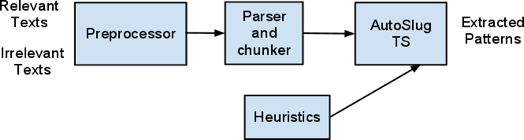
\includegraphics[scale=0.75]{workflow.png}

\begin{enumerate}

\item \textbf{Preprocessor:} Separated the metacontent from the text.
\item \textbf{Parser and NP Chunker:} We parsed the main content of the page using the Stanford parser and used the parsed tree to build a NP chunked output. 
\item \textbf{AutoSlog-TS:} We used regular expressions to look for heuristics in the chunked text and used the AutoSlog scoring mechanism to rank the extracted patterns.  
\item \textbf{Ranking formula:} $relevance rate * log2(frequency)$

\end{enumerate}

Once we had the extracted patterns we manually reviewed all of them to get a total of 99 final patterns.

\subsection*{Pattern Matching}

The following diagram shows the work-flow for the pattern matching module:


\includegraphics[scale=0.75]{patt.png}

\begin{enumerate}

\item \textbf{Preprocessor:} Splits the file into multiple texts and splits each text into meta text and main text. 
\item \textbf{Sentence-Splitter:} Splits the main text into different sentences using two patterns 1) dot followed by space or 2) dot followed by quotes.
\item \textbf{Pattern Matcher:} Uses regular expressions to match the extracted patterns for victims, targets, and perpetrators in a given sentence. For our purposes, the forward patterns were the patters in which the relevant NP occured at the beginning (e.g ``\texttt{<NP> WAS\textbackslash s*[\textbackslash w]*\textbackslash s*MURDERED}"). In contrast, backward patterns are patterns in which the relevant NP occurs at the end (e.g. ``\texttt{MURDERED <NP>}” ). We looked for forward patterns first and then for backward patterns, if a forward pattern matched then the backward pattern containing the same verb is not considered. For example, if  ``\texttt{WAS\textbackslash s*[\textbackslash w]*\textbackslash s*MURDERED}" matched then we did not look for ``\texttt{MURDERED <NP>}".
\item \textbf{Parser and NP Chunker:} If a sentence matches a particular pattern then we extract the relevant NP (i.e., for forward patterns we extract NP occurring just before the pattern and for backward patterns we extract the NP occurring after the pattern).

\end{enumerate}


\section*{Post Processor}

This module’s goal was to filter through the list of NPs returned by previous step before choosing the correct answers for each slot. We wrote methods that performed the following tasks in order to complete this module. 

\begin{enumerate}

\item \textbf{Extracting Multiple Answers from an NP:} We found that in some cases the extracted NP contained multiple answers separated by “and“, “accompanied by”, etc. We chose to look for such words and split the NP appropriately.
\item \textbf{Removing Synonyms:} We had a hard coded list of synonyms for this task. 
\item \textbf{Overlapping Answers Removal:} We often found that some of our answers overlapped (e.g., Hector Oqueli and Oqueli). In these cases, we simply chose the largest of the two strings.
\item \textbf{Appositive Removal:} Our answers for the victim slot usually contained appositives like ``Obma, President of the United States". So we maintained a list of relevant appositives and removed these if they were a part of the NP.
\item \textbf{Flag List:} We maintain flag list for all 3 of the slots. Flag list marks NPs that should be removed from consideration. For example, a victim flag list contained these words like \textit{headquarters} and \textit{embassy}. If such an NP in the list was reported, we simply removed it.
\item \textbf{Redundant word List:} This is a list of unnecessary words like verbs, weekdays, and prepositions that may be found alongside the answer, but which destroy the correctness of our answers.
\item \textbf{One word List:} This is a list of words which on their own could not be answers to any of the slots. Examples include words like \textit{headquarters}, \textit{urban}, \textit{salvador}, and so on. These words were summarily removed from any answers.

\end{enumerate}

\subsection*{Weapons Predictor}

\subsection*{Perp Org Predictor}

\section{Emphasis}

We started our project thinking that extracting the relevant patterns will be the most important part of the project, and because we did not want any bias in selecting of Patterns, we decided to go with the AutoSlug-TS approach. However we later found that the Post Processing phase was as important as the Pattern Selection phase. We were extracting a lot of irrelevant NP’s and the few relevant NP’s that we were extracting were filled with redundant words. Our most original module was the Post processor ( and Weapns ???? ) because we tried a lot of unique things in that module. However it was also the least robust part of our project.


\section{Performance Results}

TODO

\section{External Sources}

 
1.Stanford Parser : We used both Lexicalized  PCFG Parser and the normal PCFG parser.
2.Stanford NER Tagger  
3.NLTK Pos taggger 
4.TODO 

\section{Surprise Factor}

\begin{enumerate}

\item Our biggest surprise was the poor performance of the tools we used. we did not expect the parser to do as badly as it did.  
\item We had not anticipated that the post processing module to be as complicated as it was. It was really difficult to sift through all the NP’s extracted and get the correct answers.
\item Simple techniques worked better. Most people who had mined their answers from Dev set did really well, even for general slots like Victim,Targets and Perpetrator Individuals

\end{enumerate}


\section{Lessons Learned}

Overall it was a great experience to work one a real world NLP problem and to deal with real issues.

Our results in Test set 2 were bad due to over-fitting. We could have avoided this by doing the following:

\begin{enumerate}

\item Evaluating our system on an unseen data-set. 
\item Making our Post processor more robust by using machine learning techniques instead of lists.
\item Using the NER Tagger plus a dictionary( for nameless victims e.g people,child,wife etc) to validate the answers for the victim slot. 

\end{enumerate}

We could have also improved our Weapon Classifier by using the output of the incident predictor as one of the features for the weapon predictor

\section{Contribution of each Team Member}

Incident Predictor : Vishay
NP Chunker: Vishay and Alex  
AutoSlog-TS : Vishay and Alex
Pre-Processor : Vishay and Alex 
Pattern Matcher : Vishay
Parsing module : Vishay
NER Tagger module : Vishay 






\end{document}